\documentclass{beamer}

\usepackage[scale=2]{ccicons}
\usepackage{stmaryrd}
\usepackage{graphicx}
\usepackage{booktabs}
\usepackage{gensymb}

% Beamer configuration
\usetheme[sectionpage=progressbar, numbering=counter, progressbar=frametitle]{metropolis}

\usepackage{pgfplots}
\usepackage{pgfplotsthemetol}

% Progressbar
\setbeamercolor{progress bar}{
    fg=TolLightGreen,
    bg=TolLightGreen!50!black!30
}
\makeatletter
    \setlength{\metropolis@titleseparator@linewidth}{2pt}
    \setlength{\metropolis@progressonsectionpage@linewidth}{2pt}
    \setlength{\metropolis@progressinheadfoot@linewidth}{2pt}
\makeatother

% Footer
\setbeamertemplate{frame footer}{Quentin Brateau, ENSTA Bretagne}

% Block fill
\metroset{block=fill}

\title{Sea route monitoring by weather buoys using interval analysis}
\date{\today}
\author{Quentin Brateau}
\institute{ENSTA Bretagne}

\begin{document}

    \maketitle

    \section{Introduction}

        \begin{frame}{Introduction}
            \begin{minipage}{0.55\textwidth}
                \begin{block}<1->{Problem statement}
                    Estimate the state of multiples sub-systems governed by the same evolution equation.
                \end{block}
                \begin{block}<2->{Measurements}
                    Sub-systems are sensed by independant sensors. The number of sensors can be significant.
                \end{block}
            \end{minipage}
            \hfill
            \onslide<3->
            \begin{minipage}{0.4\textwidth}
                \begin{figure}
                    \includegraphics[width=\textwidth]{build/imgs/introduction}
                    \caption{Multiple systems sensed by multiples sensors}
                \end{figure}
            \end{minipage}
        \end{frame}

    \section{Formalism}

        \begin{frame}{State eqaution}
            \begin{block}<1->{Evolution equation}
                $\forall n \in \mathbb{N}$ the number of systems, $\forall i \in \llbracket 1, n\rrbracket$, $\mathbf{x_i}$ is the state of the $i^{th}$ system such that
                \begin{equation}
                    \dot{\mathbf{x_i}} = f(\mathbf{x_i})
                \end{equation}
            \end{block}

            \begin{block}<2->{Measurement equation}
                $\forall m \in \mathbb{N}$ the number of sensors, $\forall k \in \llbracket 1, m\rrbracket$, $\exists j \in \llbracket 1, n\rrbracket$ such that
                \begin{equation}
                    g^k(\mathbf{x_i}(t_j)) \in \mathbb{Y}_j^k
                \end{equation}
            \end{block}
        \end{frame}

        \begin{frame}{Combinatorial approach}
            \begin{block}<1->{Combinatorial approach}
                $\forall n \in \mathbb{N}$ the number of boats, $\forall m \in \mathbb{N}$ the number of sensors, there is $d = n^m$ detections.
            \end{block}
            \begin{exampleblock}<2->{Example}
                With $n = 5$ boats and $m = 20$ sensors,
                $$d = n^m = 5^{20} = 9.5e^{13}$$
            \end{exampleblock}
        \end{frame}

        \begin{frame}{Proposed approach}
            \begin{block}<1->{Proposed approach}
                \begin{quote}
                    \centering
                    Any detection could be produced by any sub-system.
                \end{quote}
                $\forall n \in \mathbb{N}$ the number of boats, $\forall m \in \mathbb{N}$ the number of sensors, there is $d = n \times m$ detections.
            \end{block}
            \begin{exampleblock}<2->{Example}
                With $n = 5$ boats and $m = 20$ sensors,
                $$d = n \times m = 5 \times 20 = 120$$
            \end{exampleblock}
        \end{frame}

        \begin{frame}{Detection space}
            \begin{block}<1->{Sensor detection set}
                $\forall k \in \llbracket 1, m\rrbracket$, $\mathbb{Y}^k$ is the detection set of the $k^{th}$ sensor such that
                \begin{equation}
                    \mathbb{Y}^k = \bigcup_{j \in \llbracket 1, m\rrbracket} \mathbb{Y}_j^k
                \end{equation}
            \end{block}
            \begin{block}<2->{Detection space}
                $\mathbb{Y} \in \mathbb{R}^k$ is the detection set of all the systems such that
                \begin{equation}
                    \mathbb{Y} = \mathbb{Y}^1 \times \dots \times \mathbb{Y}^m
                \end{equation}
            \end{block}
        \end{frame}

        \begin{frame}{Example}
            \begin{exampleblock}<1->{Example}
                Assuming that $n = 3$, $m = 2$, and
                $$\forall k \in \llbracket 1, m\rrbracket, \;  \forall j \in \llbracket 1, m\rrbracket, \quad \mathbb{Y}_k^j \in \mathbb{R}$$
            \end{exampleblock}
            \begin{exampleblock}<2->{Detection space}
                Then $\mathbb{Y} \in \mathbb{R}^2$ and
                \begin{eqnarray}
                    \mathbb{Y} & = & \mathbb{Y}^1 \times \mathbb{Y}^2 \\
                    & = & \left(\mathbb{Y}_1^1 \cup \mathbb{Y}_2^1 \cup \mathbb{Y}_3^1\right) \times \left(\mathbb{Y}_1^1 \cup \mathbb{Y}_2^1 \cup \mathbb{Y}_3^1\right)
                \end{eqnarray}
            \end{exampleblock}
        \end{frame}

        \begin{frame}{Example}
            \begin{minipage}{0.45\textwidth}
                \begin{table}
                    \begin{tabular}{@{} rcc @{}}
                        \toprule
                        & $s_1$ & $s_2$ \\
                        \midrule
                        $\mathbb{Y}_1$ & $\lbrack0.97, 1.97\rbrack$ & $\lbrack1.51, 2.51\rbrack$  \\
                        $\mathbb{Y}_2$ & $\lbrack3.18, 4.18\rbrack$ & $\lbrack4.01, 1.01\rbrack$ \\
                        $\mathbb{Y}_3$ & $\lbrack6.62, 7.62\rbrack$ & $\lbrack6.47, 6.47\rbrack$ \\
                        \bottomrule
                    \end{tabular}
                    \caption{Detection times}
                \end{table}
            \end{minipage}
            \hfill
            \begin{minipage}{0.5\textwidth}
                \begin{figure}
                    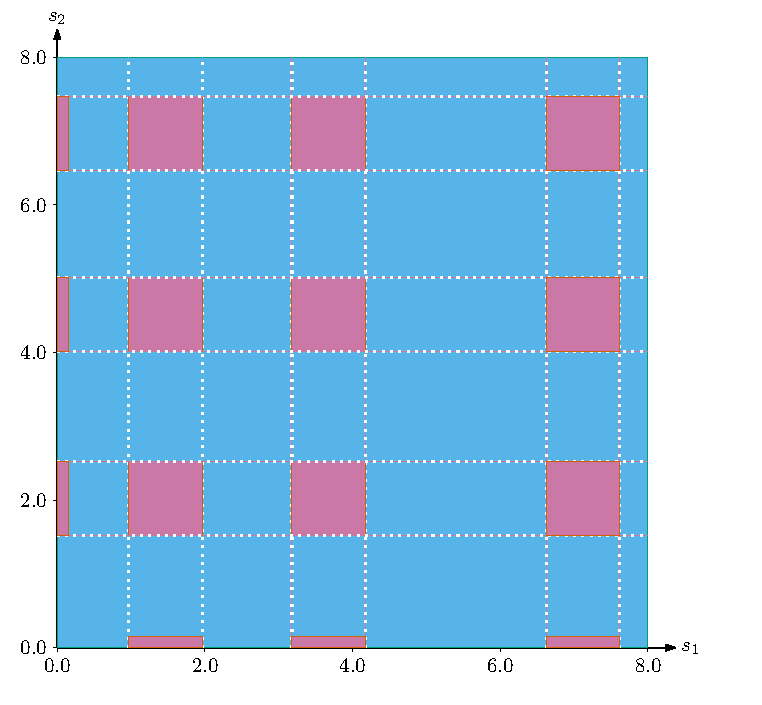
\includegraphics[height=0.7\textheight]{imgs/detection_space}
                    \caption{Detection space}
                \end{figure}
            \end{minipage}
        \end{frame}

        \begin{frame}{State estimation}
            \begin{block}<1->{Set inversion}
                The state of the system is estimated using set inversion algorithm.
                \begin{equation}
                    \mathbb{X} = \lbrace x \in \mathbb{R}^k \mid\ f(x) \in \mathbb{Y}\rbrace
                \end{equation}
            \end{block}
        \end{frame}

    \section{Application: Sea route monitoring}

        \begin{frame}{Boat wake}
            \centering
            \begin{minipage}{0.6\textwidth}
                \begin{block}{Wake's angle}
                    \begin{equation}
                        \alpha = \arcsin\left(\frac{1}{3}\right) \approx 19.47 \degree
                    \end{equation}
                \end{block}
                \vspace{0.2cm}
                \begin{figure}
                    \centering
                    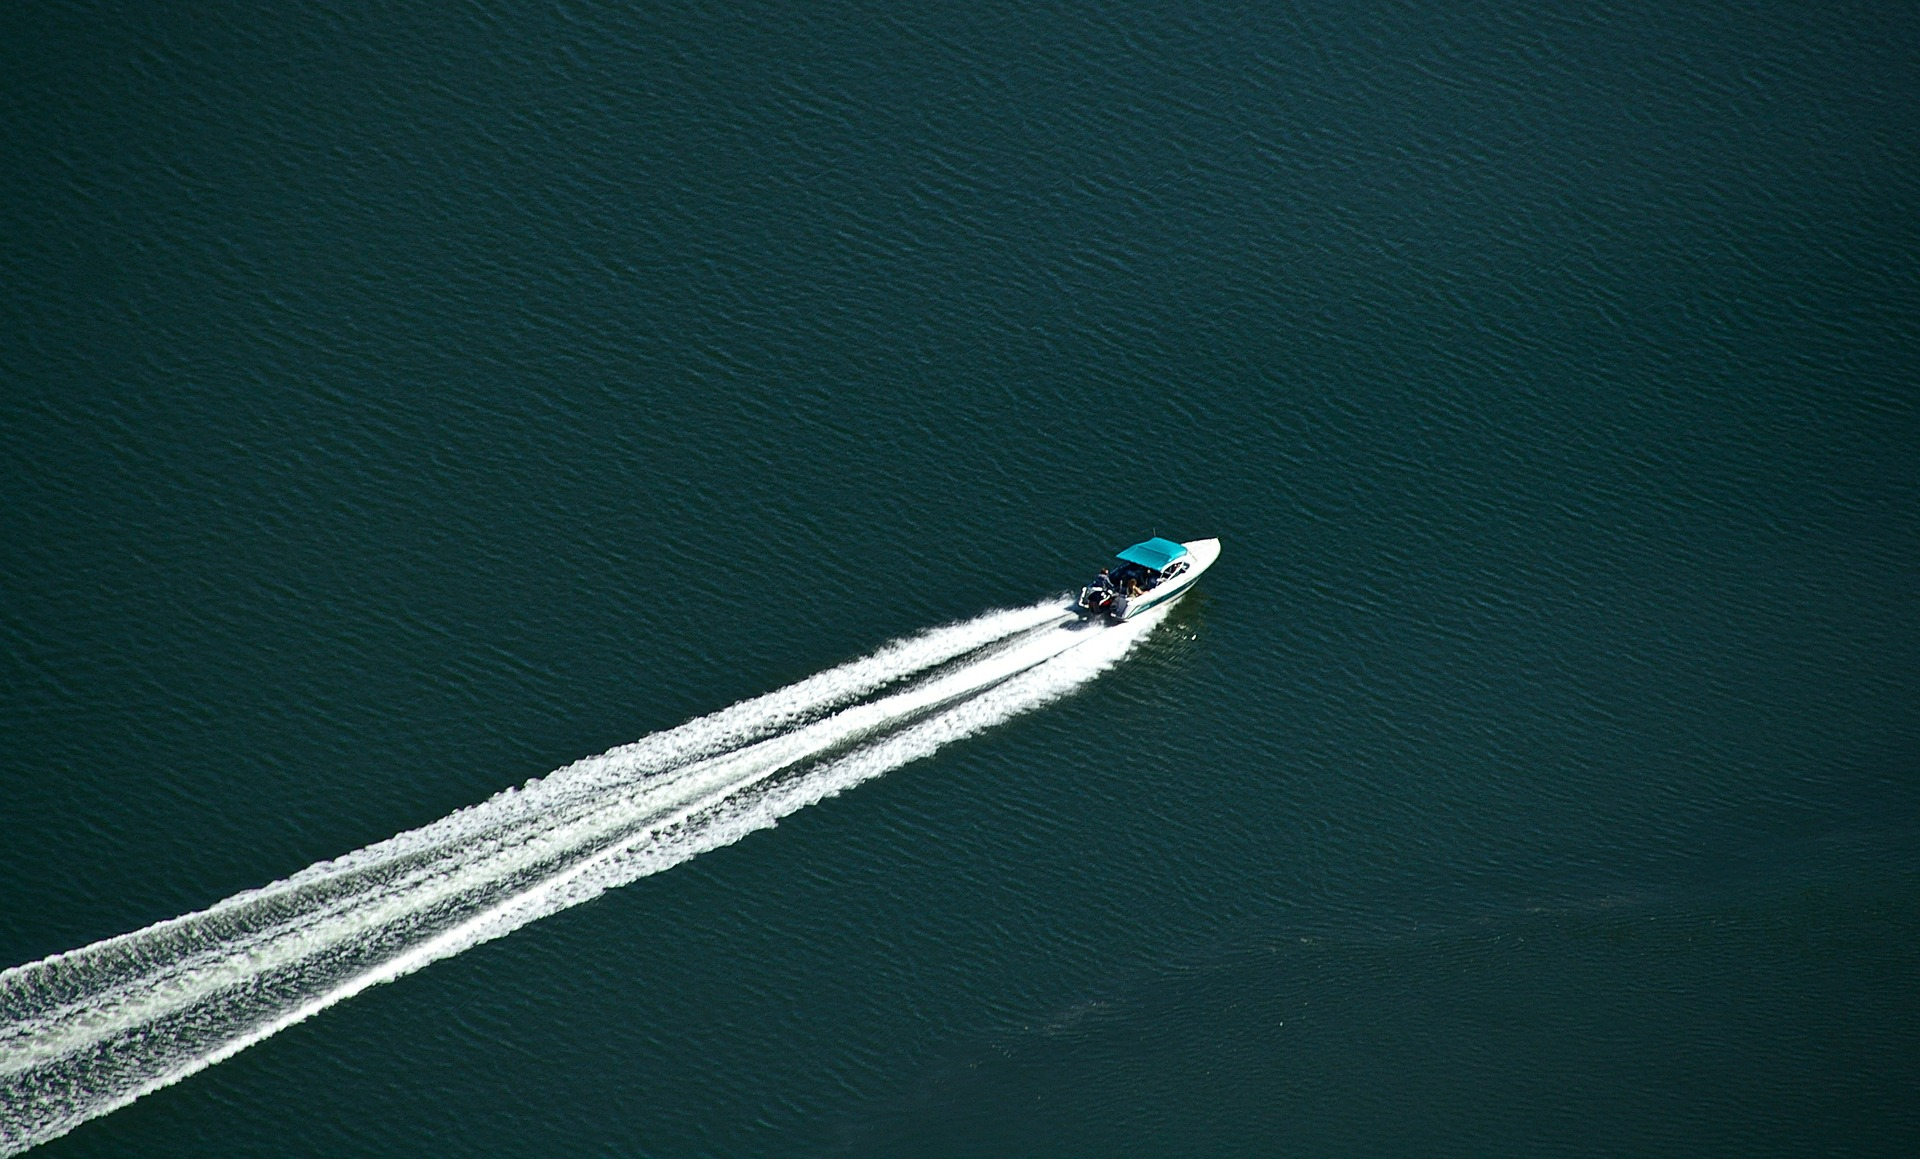
\includegraphics[width=\textwidth,trim={0 0 17cm 14cm},clip]{imgs/motorboat}
                    \caption{Boat and wake}
                \end{figure}
            \end{minipage}
        \end{frame}

        \begin{frame}{Formalism}
            \begin{block}<1->{Boat's state}
                Assuming each boats are moving straight ahead along the x-axis
                $$\forall i \in \llbracket 1, n\rrbracket, \quad \mathbf{x_i} = (x_i, y_i, v_i)^T$$ 
            \end{block}

            \begin{block}<2->{State equation}
                \begin{eqnarray}
                    f:& \mathbf{x_i} &\mapsto (v_i.dt, 0, 0)^T \\
                    g^k:& \mathbf{x_i}  &\mapsto \frac{1}{v_i} \left(\frac{y_i - y^k}{tan(\alpha)} - (x_i - x^k)\right)
                \end{eqnarray}
            \end{block}
        \end{frame}

        \begin{frame}{Example one boat}
            \begin{minipage}{0.45\textwidth}
                \begin{figure}
                        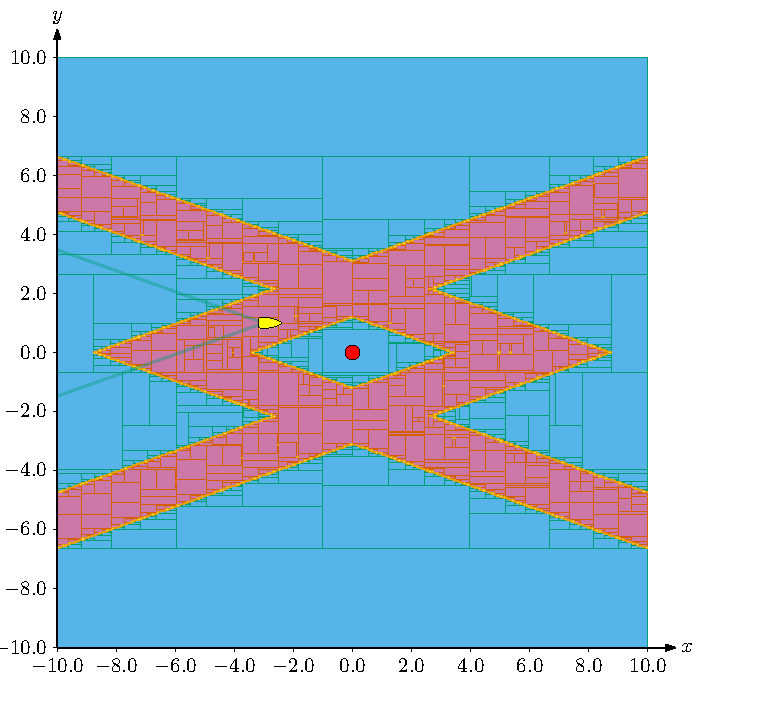
\includegraphics[width=\textwidth]{imgs/forward}
                        \caption{Forward boat detection set $\mathbb{Y}_1^1 = \lbrack3.38, 4.38\rbrack s$}
                \end{figure}
            \end{minipage}
            \hfill
            \begin{minipage}{0.45\textwidth}
                \begin{figure}
                        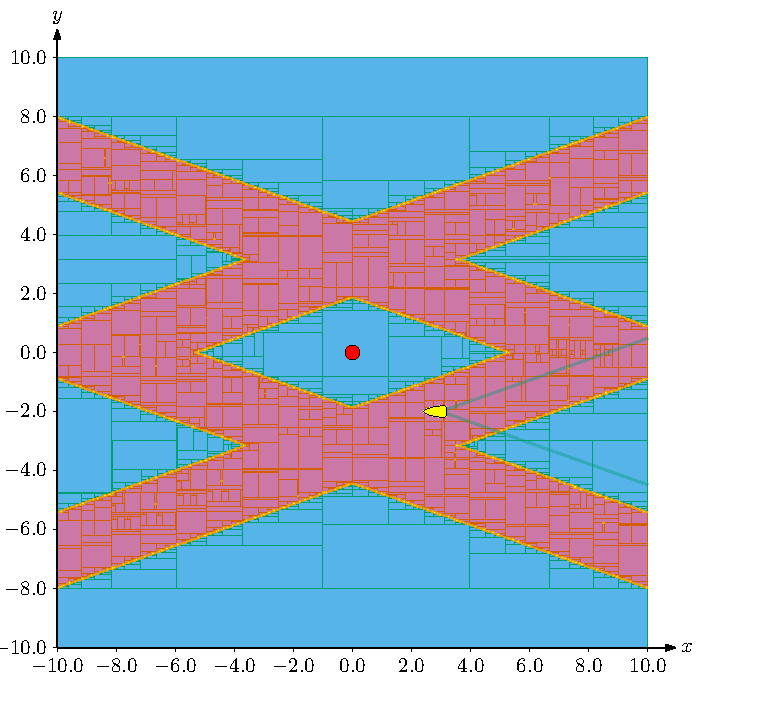
\includegraphics[width=\textwidth]{imgs/backward}
                        \caption{Backward boat detection set $\mathbb{Y}_1^1 = \lbrack5.26, 6.26\rbrack s$}
                \end{figure}
            \end{minipage}
        \end{frame}

        \begin{frame}{Example two sensors}
            \begin{minipage}{0.45\textwidth}
                \begin{figure}
                        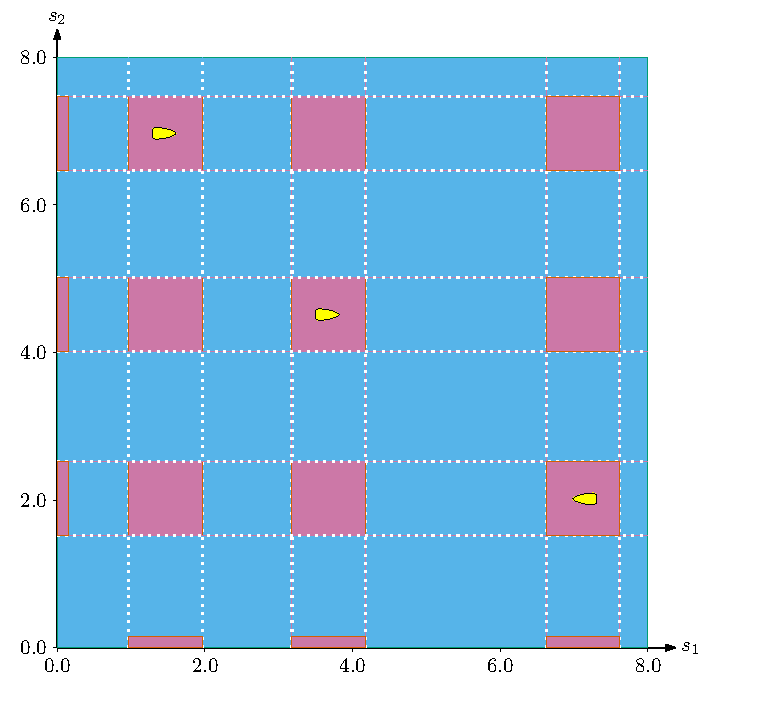
\includegraphics[width=\textwidth]{imgs/ex_detection_space}
                        \caption{Detection space}
                \end{figure}
            \end{minipage}
            \hfill
            \begin{minipage}{0.45\textwidth}
                \begin{figure}
                        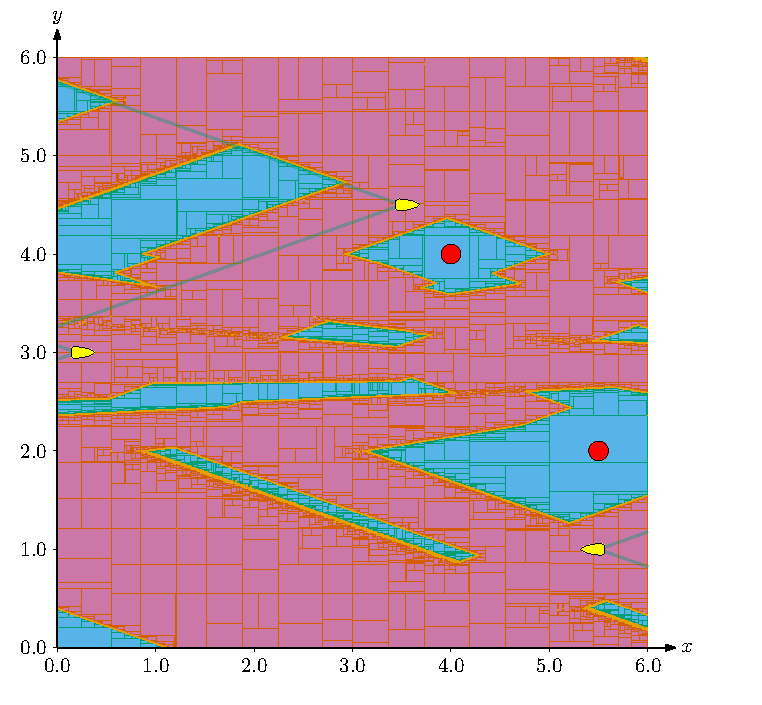
\includegraphics[width=\textwidth]{imgs/ex_boat_space}
                        \caption{Boat space}
                \end{figure}
            \end{minipage}
        \end{frame}

        \begin{frame}{Causal approach}
            
        \end{frame}

        \begin{frame}{Acausal approach}
            
        \end{frame}

    \section{Conclusion}
\end{document}